
\section{\trMorseHomology{}的\trFunctoriality}
\label{sec:functoriality}

我们已经看到（即\cref{thm:diffeomorphism-homology}）：两个\trManifold{}之间的\trDiffeomorphism{}在\trMorseHomology{}的层面上诱导一个\trIsomorphism。更一般地，我们想要证明：一个 $\cC^\infty$ 映射诱导一个\textbf{\trHomomorphism}（homomorphism）。遗憾的是，仅有一条映射 $u\colon V\to W$ 并不足以从 $W$ 上的一个\trMorseFunction{}构造出 $V$ 上的\trMorseFunction，因此我们将不得不做得更精巧一些。

我们这里所考虑的\trManifold{} $V$ 是一个\trCompact\trManifold，可能带边界，其上赋予了一个\trMorseFunction{} $f$ 与一个满足\trSmale{}性质的\trPseudogradient{}场 $X$；并且当 $\partial V\neq\varnothing$ 时，这个场还是\trIncoming{}的（沿用先前的记号，$\partial V=\partial_-V$）。

我们在这里将要证明的结果，是下面这两个定理。

\begin{theorem}[\trFunctoriality]\label{thm:functoriality}
设 $u\colon V\to W$ 是一个 $\cC^\infty$ 类的映射。它诱导\textbf{\trGraded\trAbelianGroup}（graded abelian groups）之间的一个\trMorphism
\[
u_\star\colon HM_\star(V)\longrightarrow HM_\star(W)\text{。}
\]
此外，若 $v\colon W\to Z$ 是另一个 $\cC^\infty$ 映射，则
\[
(v\circ u)_\star=v_\star\circ u_\star\text{。}
\]
最后，对恒等映射 $\mathrm{Id}\colon V\to V$，我们有 $\mathrm{Id}_\star=\mathrm{Id}$。
\end{theorem}

说 $u_\star$ 是\trGraded\trAbelianGroup{}之间的一个\trMorphism，即是说这个映射是一族\trMorphism
\[
u_k\colon HM_k(V)\longrightarrow HM_k(W)\text{。}
\]

用术语来说，这个定理断言：\trMorseHomology{}是从\trDifferential\trManifold{}与 $\cC^\infty$ 映射的\textbf{\trCategory}（category）到\trAbelianGroup{}的\trCategory{}之中的一个\textbf{\trFunctor}（functor）。它还是一个“\trHomotopy”\trFunctor。

\begin{theorem}[\trHomotopy{}不变性]\label{thm:homotopy-invariance}
设 $u\colon[0,1]\times V\to W$ 是一个 $\cC^\infty$ 映射。对 $u_t(x)=u(t,x)$，我们有 $(u_0)_\star=(u_1)_\star$。
\end{theorem}

\cref{thm:functoriality}的证明想法，是利用这样一个事实：复合
\[
V\xrightarrow{\ \ u\ \ }W=W\times\{0\}\subset W\times D^N
\]
与一个\trEmbedding{}是\trHomotopic{}的（对充分大的 $N$），因此我们先从\trEmbedding{}的情形做起。

\begin{proof}[\cref{thm:functoriality}的证明（\trEmbedding{}情形）]
设在 $V$ 上给定一个具有\trMorse{}性质与\trSmale{}性质的对 $(f,X)$，想法是把它延拓成 $W$ 上一个具有同样性质的对 $(\widetilde f,\widetilde X)$。由它我们将导出一个\trComplex{}\trMorphism
\[
u_\bullet\colon C_\bullet(f,X)\longrightarrow C_\bullet(\widetilde f,\widetilde X)\text{。}
\]
随后我们将证明：它在\trHomology{}上诱导的\trMorphism{}不依赖于 $f$ 与 $X$ 的选取。

\emph{$u$ 为\trDiffeomorphism{}的情形。}

我们在\cref{thm:diffeomorphism-homology}中已经看到，\trDiffeomorphism{} $u$ 诱导\trComplex{}的一个\trIsomorphism
\[
C_\bullet(f,X)\longrightarrow C_\bullet(f\circ u^{-1},du(X))\text{。}
\]
让我们验证一下：在\trHomology{}上诱导的\trIsomorphism{}不依赖于 $f$ 与 $X$ 的选取。于是，设 $(f_0,X_0)$ 与 $(f_1,X_1)$ 是 $V$ 上的两个\trMorse--\trSmale{}对，并设 $(F,X)$ 是 $[-1/3,4/3]\times V$ 上的一个\trMorse--\trSmale{}对，如\cref{sec:homology-independence}中那样。对 $(f_0\circ u^{-1},du(X_0))$ 与 $(f_1\circ u^{-1},du(X_1))$ 而言，扮演同样角色的正是对 $(F\circ(\mathrm{Id}\times u^{-1}),d(\mathrm{Id}\times u)(X))$。换言之，我们有下面这幅交换图。
\[
\begin{tikzcd}[column sep=1.7cm,row sep=1.55cm]
C_\bullet(f_0,X_0) \ar[r,"u_{\bullet 0}"] \ar[d,"\Phi^F"']
  & C_\bullet(f_0\circ u^{-1},du(X_0)) \ar[d,"\Phi^{F\circ(\mathrm{Id}\times u^{-1})}"] \\
C_\bullet(f_1,X_1) \ar[r,"u_{\bullet 1}"']
  & C_\bullet(f_1\circ u^{-1},du(X_1))
\end{tikzcd}
\]
显然，对两个\trDiffeomorphism{} $u$ 与 $v$，我们有 $v_\bullet\circ u_\bullet=(v\circ u)_\bullet$，从而 $v_\star\circ u_\star=(v\circ u)_\star$。最后，$\mathrm{Id}_\star=\mathrm{Id}$。

\emph{$u$ 为往一个\trSubmanifold{}作包含的情形。}

让我们把它记作
\[
i\colon V\hookrightarrow W\text{。}
\]

\begin{proposition}\label{thm:morse-smale-extension}
设 $(f,X)$ 是 $V$ 上的一个\trMorse--\trSmale{}对。那么存在 $W$ 上一个延拓它的\trMorse--\trSmale{}对 $(\widetilde f,\widetilde X)$，满足：
\begin{enumerate}[label=(\arabic*)]
\item $\operatorname{Crit}(f)\subset\operatorname{Crit}(\widetilde f)$，且 $f$ 的一个\trCriticalPoint{}的\trIndex{}与它作为 $\widetilde f$ 的\trCriticalPoint{}的\trIndex{}相同；
\item 若 $a$ 是 $f$ 的一个\trCriticalPoint，则 $\partial_{\widetilde X}(a)=\partial_X(a)$。\footnote{译注：原书对 $V$ 往 $W$ 的任意\trSubmanifold{}包含一律照此陈述（含像落在带边目标 $W$ 的边界 $\partial W$ 上的情形），照排于此；按本证明的构造（在 $U\equiv D^n\times D^{p-n}$ 上延拓并要求场沿边界\trIncoming），若\trEmbedding{}的像落在 $\partial W$ 上或触及 $\partial W$，延拓便与\trIncoming{}条件相抵；严格表述须先设\trEmbedding{}的像落在 $W$ 的内部，或先给目标添一层\trCollar{}再作延拓。——译者注}
\end{enumerate}
\end{proposition}

作为这条命题的一个推论，我们便有一个（\trInjective{}的）\trComplex\trMorphism
\[
i_\bullet\colon C_\bullet(f,X)\longrightarrow C_\bullet(\widetilde f,\widetilde X)
\]
它的定义无非是把 $a$（视为 $f$ 的\trCriticalPoint）送到 $a$（视为 $\widetilde f$ 的\trCriticalPoint）。此外，这个\trMorphism{}不依赖于对 $(f,X)$ 的选取：我们照常把 $(f_0,X_0)$ 连接到 $(f_1,X_1)$，利用一个函数
\[
F\colon[-1/3,4/3]\times V\longrightarrow\RR
\]
和这个乘积上的一个\trVectorField{} $X$。我们可以作出下面这幅交换图
\[
\begin{tikzcd}[column sep=1.15cm,row sep=1.55cm]
C_\bullet(f_0,X_0) \ar[r,hook,"u_{\bullet 0}"] \ar[d,"\Phi^F"']
  & C_\bullet(\widetilde f_0,\widetilde X_0) \ar[d,"\Phi^{\widetilde F}"] \\
C_\bullet(f_1,X_1) \ar[r,hook,"u_{\bullet 1}"']
  & C_\bullet(\widetilde f_1,\widetilde X_1)
\end{tikzcd}
\]
只需把 $F$ 与 $X$ 延拓成 $\widetilde F$ 与 $\widetilde X$，正如我们延拓 $f$ 与 $X$ 那样，于是若 $a$ 是 $f_0$ 在 $V$ 上的一个\trCriticalPoint，则 $\Phi^{\widetilde F}(a)=\Phi^F(a)$。

\emph{$u\colon V\to W$ 为\trEmbedding{}的情形。}

我们可以把 $u$ 看作一个\trDiffeomorphism{}与往一个\trSubmanifold{}作包含的复合：
\[
V\xrightarrow{\;u\;}u(V)\xhookrightarrow{\;i\;}W\text{。}
\]
从 $V$ 上的 $(f,X)$ 出发，我们像上面那样构造出 $W$ 上的 $(\widetilde f,\widetilde X)$ 以及一个\trComplex\trMorphism
\[
u_\bullet\colon C_\bullet(f,X)\longrightarrow C_\bullet(\widetilde f,\widetilde X)
\]
办法是把 $a$ 送到 $iu(a)=u(a)$。

我们显然有
\[
v_\bullet\circ u_\bullet=(v\circ u)_\bullet\text{，从而也有 }v_\star\circ u_\star=(v\circ u)_\star\text{。}\qedhere
\]
\end{proof}

\begin{proof}[\cref{thm:morse-smale-extension}的证明]
让我们来考察\trManifold{} $W$ 的一个维数为 $n$ 的\trSubmanifold{} $V$，其中 $W$ 的维数为 $p$。设 $c$ 是 $f$ 在 $V$ 上的一个\trCriticalPoint，并设 $U$ 是 $c$ 在（更大的）\trManifold{} $W$ 中的一个邻域。我们可以——而且我们也确实——假定 $U$ 形如 $U\equiv D^n\times D^{p-n}$。在这样一个 $U$ 上，容易延拓 $f$：令
\[
\widetilde f(x,y)=f(x)+\frac{1}{2}\,\|y\|^2
\]
并延拓 $X$：令
\[
\widetilde X(x,y)=X(x)-y
\]
（也就是说，给 $X(x)$ 添上范数的平方的负\trGradient）。于是，对 $f$ 的每个\trCriticalPoint{} $c_i$，我们都选取这样一个邻域 $U_i$，并延拓 $f$ 与 $X$：在诸 $U_i$ 上固定这个形状，而在 $W$ 中诸 $U_i$ 之并的补集上任意地延拓它。

\setcounter{figure}{2}%
\begin{figure}[htbp]
\centering
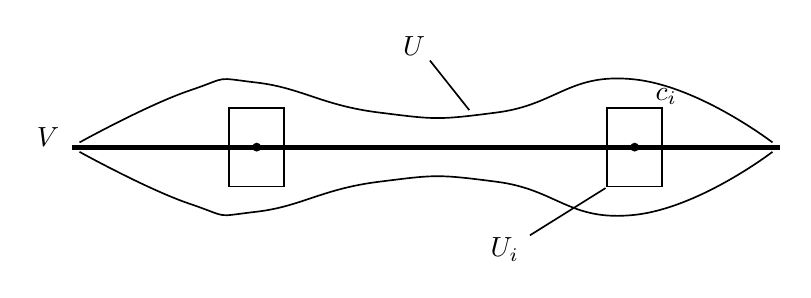
\begin{tikzpicture}[line width=0.6pt]
  \draw[line width=1.9pt] (0,0) -- (9,0);
  \node at (-0.3,0.13) {$V$};
  \draw plot[smooth,tension=0.85] coordinates{
    (0.1,0.06) (1.5,0.72) (2.35,0.82) (3.9,0.44) (5.4,0.44) (7.15,0.86) (8.9,0.06)};
  \draw plot[smooth,tension=0.85] coordinates{
    (0.1,-0.06) (1.5,-0.72) (2.35,-0.82) (3.9,-0.44) (5.4,-0.44) (7.15,-0.86) (8.9,-0.06)};
  \draw (2.0,-0.5) rectangle (2.7,0.5);
  \fill (2.35,0) circle (1.6pt);
  \draw (6.8,-0.5) rectangle (7.5,0.5);
  \fill (7.15,0) circle (1.6pt);
  \node at (7.55,0.64) {$c_i$};
  \node at (4.35,1.28) {$U$};
  \draw (4.55,1.1) -- (5.05,0.47);
  \node at (5.5,-1.3) {$U_i$};
  \draw (5.82,-1.12) -- (6.78,-0.52);
\end{tikzpicture}
\caption{}
\label{fig:critical-neighborhoods-extension}
\end{figure}

由于 $f$ 在 $V$ 上的所有\trCriticalPoint{}都含于诸 $U_i$ 之中，而 $X$ 是一个\trPseudogradient，故存在一个 $\varepsilon_0>0$，使得
\[
d\widetilde f(\widetilde X)<-\varepsilon_0
\]
在 $V-\cup(U_i\cap V)$ 上并且在诸 $U_i$ 的边界附近都成立。于是，存在 $V\cup(\cup U_i)$ 在 $W$ 中的一个\trOpen{}邻域 $U$，使得
\[
d\widetilde f(\widetilde X)\le 0
\]
在 $U$ 上成立，而等号恰好在诸 $c_i$ 处取得。

特别地，在 $U$ 上，$\widetilde f$ 除了诸 $c_i$ 之外没有别的\trCriticalPoint。由于我们给 $f$ 添上了一个\trPositiveDefinite\trQuadraticForm，$c$ 作为 $\widetilde f$ 的\trCriticalPoint{}的\trIndex{}就是它作为 $f$ 的\trCriticalPoint{}的\trIndex。

没有任何理由指望：这样任意延拓 $f$ 所得到的 $\widetilde f$ 在 $U$ 之外会是\trMorseFunction。因此我们取一个微小的\trPerturbation，使之成为\trMorseFunction。随后，我们利用一个\trPartitionOfUnity，构造出 $X$ 到一个\trPseudogradient{} $\widetilde X$ 的一个\emph{合适}的延拓。

\begin{remark}\label{thm:trajectory-contained-in-v}
请注意，$\widetilde X$ 的每一条满足 $\lim_{t\to-\infty}\gamma(t)=c\in V$ 的\trTrajectory{}都完全含于 $V$ 之中（我们已经假定 $X$ 在 $\partial V$ 附近是\trIncoming{}的）。

延拓后的场 $\widetilde X$ 未必拥有\trSmale{}性质。不过，对 $f$ 的所有\trCriticalPoint，我们仍然有 $\mathcal{L}_{\widetilde X}(a,b)=\mathcal{L}_X(a,b)$，于是
\[
n_{\widetilde X}(a,b)=n_X(a,b)\text{，从而 }\partial_{\widetilde X}(a)=\partial_X(a)\text{。}
\]

如果 $\widetilde X$ 确实拥有\trSmale{}性质，那么我们就得到了预期中的结果。必要时对 $\widetilde X$ 作一个\trPerturbation，我们便得到一个非常贴近并且满足\trSmale{}性质的场。它可能不再与 $V$ 相切，但它仍然满足 $n_{\widetilde X}(a,b)=n_X(a,b)$。
\end{remark}
\end{proof}

\begin{remark}\label{thm:tubular-neighborhood-homology}
请特别注意，应用这个证明即可表明：若 $V$ 是一个\trManifold{} $W$ 的\trSubmanifold，而 $\mathcal{V}$ 是 $V$ 在 $W$ 中的一个\trTubularNeighborhood，则 $HM_\star(\mathcal{V})\cong HM_\star(V)$。
\end{remark}

在结束\cref{thm:functoriality}的证明（非\trEmbedding{}映射的一般情形）之前，让我们先着手证明\cref{thm:homotopy-invariance}，它日后会派上用场。

\begin{proof}[\cref{thm:homotopy-invariance}的证明（\trEmbedding{}情形）]
首先注意，由于
\[
HM_\star(D^N;\ZZ)=
\begin{cases}
\ZZ & \text{若 }\star=0\\
0 & \text{其余情形}
\end{cases}
\]
对每个\trDiffeomorphism{} $\psi\colon D^N\to D^N$，映射 $\psi_\star$——它必定是 $\ZZ$ 的一个\trIsomorphism——只能是恒等映射或其负映射，也就是说 $\psi_\star=\pm\mathrm{Id}$。此外，当 $\psi$ 保持\trOrientation{}时，它就是恒等映射。

于是，对每个\trManifold{} $V$ 与每个保持 $D^N$ 的\trOrientation{}的\trDiffeomorphism{} $\psi$，映射 $\psi\times\mathrm{Id}\colon D^N\times V\to D^N\times V$ 在\trHomology{}上也诱导恒等映射，这是因为在\trComplex{}的\trTensorProduct{}上 $(\psi\times\mathrm{Id})_\bullet=\psi_\bullet\otimes\mathrm{Id}_\bullet$，从而 $(\psi\times\mathrm{Id})_\star=\psi_\star\otimes\mathrm{Id}_\star=\mathrm{Id}$。

现在让我们考虑把 $V$ \trEmbedding{}到 $D^N\times V$ 之中的几种不同方式。

\begin{lemma}\label{thm:inclusion-induced-isomorphism}
设 $a\in D^N$，并设 $i_a\colon V\to D^N\times V$ 是由 $i_a(x)=(a,x)$ 定义的\trEmbedding。那么：
\begin{enumerate}[label=(\arabic*)]
\item $(i_0)_\star$ 是一个\trIsomorphism；
\item $(i_a)_\star=(i_0)_\star$。\footnote{译注：原书设 $a\in D^N$，照排于此；但证明中所用的\trDiffeomorphism{} $\psi\colon D^N\to D^N$ 保持边界，只能把内点 $0$ 送到内点，故 $a$ 应限于 $D^N$ 的内点（这与证明脚注所引练习~19 在\trOpen{}\trDisk{}上构造流的口径一致）；$a$ 为边界点时断言本身仍真，但严格论证须另走\trHomotopy{}之路，而本书行文至此处尚无\trHomotopy{}不变性可用。——译者注}
\end{enumerate}
\end{lemma}

\begin{proof}
我们取 $V$ 上的一个\trMorse--\trSmale{}对 $(f,X)$，这里 $V$ 已与 $\{0\}\times V\subset D^N\times V$ 等同。我们像先前那样把 $(f,X)$ 延拓为 $(\widetilde f,\widetilde X)$，也就是说，令
\[
\widetilde f(y,x)=\frac{1}{2}\,\|y\|^2+f(x)
\qquad\text{和}\qquad
\widetilde X(y,x)=-y+X(x)\text{。}
\]
于是 $C_\bullet(f,X)=C_\bullet(\widetilde f,\widetilde X)$，从而 $(i_0)_\bullet=\mathrm{Id}$。这就证明了第一条断言。对于第二条，我们使用一个把 $0$ 送到 $a$ 的\trDiffeomorphism\footnote{这样一个\trDiffeomorphism{}的存在性，可以通过积分\trDisk{} $D^N$ 上一个合适的\trVectorField{}来证明；这个练习的细节留给读者（\cref{ex:ch04-19}）。} $\psi\colon D^N\to D^N$。交换图
\[
\begin{tikzcd}[column sep=1.25cm,row sep=1.35cm]
V \ar[r,hook,"i_0"] \ar[dr,hook,"i_a"'] & D^N\times V \ar[d,"\psi\times\mathrm{Id}"] \\
& D^N\times V
\end{tikzcd}
\]
给出 $(i_0)_\star=(i_a)_\star$，这正是所要证的。
\end{proof}

为了证明\trHomotopy{}不变性定理（\cref{thm:homotopy-invariance}）的这个特殊情形，我们于是考虑一个映射
\[
u\colon[0,1]\times V\longrightarrow W
\]
使得每个 $u_t$ 都是一个\trEmbedding。那么
\[
\begin{aligned}
\widetilde u\colon[0,1]\times V &\longrightarrow[0,1]\times W\\
(t,x) &\longmapsto(t,u_t(x))
\end{aligned}
\]
是一个\trEmbedding。对于包含 $i_0$ 与 $i_1$（该引理的记号），我们有两幅交换图：
\[
\begin{tikzcd}[column sep=1.15cm,row sep=1.35cm]
{[0,1]\times V} \ar[r,"\widetilde u"] & {[0,1]\times W} \\
V \ar[u,"i_0^V"] \ar[r,"u_0"'] & W \ar[u,"i_0^W"']
\end{tikzcd}
\qquad
\begin{tikzcd}[column sep=1.15cm,row sep=1.35cm]
{[0,1]\times V} \ar[r,"\widetilde u"] & {[0,1]\times W} \\
V \ar[u,"i_1^V"] \ar[r,"u_1"'] & W \ar[u,"i_1^W"']
\end{tikzcd}
\]
由它们我们推出
\[
(u_0)_\star=(i_0^W)_\star^{-1}\circ\widetilde u_\star\circ(i_0^V)_\star
  =(i_1^W)_\star^{-1}\circ\widetilde u_\star\circ(i_1^V)_\star=(u_1)_\star\text{。}\qedhere
\]
\end{proof}

\begin{proof}[\cref{thm:functoriality}的证明（一般情形）]
考虑一个 $\cC^\infty$ 类的映射：
\[
u\colon V\longrightarrow W\text{。}
\]
我们选取一个充分大的整数 $N$，使得存在一个\trEmbedding{} $\varphi\colon V\to D^N$。于是 $(\varphi,u)$ 是 $V$ 在 $D^N\times W$ 中的一个\trEmbedding。我们考虑图
\[
\begin{tikzcd}[column sep=1.5cm,row sep=1.45cm]
& D^N\times W \\
V \ar[ur,"{(\varphi,u)}"] \ar[r,"u"'] & W \ar[u,"i_0"']
\end{tikzcd}
\]
并令
\[
u_\star=(i_0)_\star^{-1}\circ(\varphi,u)_\star\text{。}
\]

让我们证明：如此得到的\trMorphism{} $u_\star$ 既不依赖于 $N$ 的选取，也不依赖于 $\varphi$（这样一来，特别地，若 $u$ 是一个\trEmbedding，则在 $N=0$ 时我们就会重新找到先前已经构造出的那个\trMorphism）。于是，我们再考虑另一个映射 $\psi\colon V\to D^M$ 与图
\[
\begin{tikzcd}[column sep=1.05cm,row sep=1.55cm]
 & D^N\times W \ar[dr,"\ell_0"] & \\
 W \ar[ur,"i_0"] \ar[dr,"j_0"']
   & V \ar[l,"u"'] \ar[u,"{(\varphi,u)}"'] \ar[r,"{(\psi,\varphi,u)}"] \ar[d,"{(\psi,u)}"']
   & D^M\times D^N\times W \\
 & D^M\times W \ar[ur,"k_0"'] &
\end{tikzcd}
\]
其中 $\ell_0$ 与 $k_0$ 定义为
\[
\ell_0(y,x)=(0,y,x)
\qquad\text{而}\qquad
k_0(z,x)=(z,0,x)\text{。}
\]
我们有 $k_0\circ j_0=\ell_0\circ i_0$，但图中右边的两个三角形并不交换。不过，在\trHomology{}上诱导出的诸图却是交换的。\trHomotopy{}“$t\psi$”连接着
\[
\ell_0(\varphi(x),u(x))=(0,\varphi(x),u(x))
\qquad\text{与}\qquad
(\psi(x),\varphi(x),u(x))
\]
同样地，\trHomotopy{}“$t\varphi$”连接着
\[
k_0(\psi(x),u(x))=(\psi(x),0,u(x))
\qquad\text{与}\qquad
(\psi(x),\varphi(x),u(x))\text{。}
\]
利用这幅图与这些评注，现在让我们来研究映射 $(i_0)_\star^{-1}\circ(\varphi,u)_\star$。我们得到
\[
\begin{aligned}
(i_0)_\star^{-1}\circ(\varphi,u)_\star
  &=(i_0)_\star^{-1}\circ(\ell_0)_\star^{-1}\circ(\psi,\varphi,u)_\star\\
  &=(j_0)_\star^{-1}\circ(k_0)_\star^{-1}\circ(\psi,\varphi,u)_\star\\
  &=(j_0)_\star^{-1}\circ(\psi,u)_\star\text{。}
\end{aligned}
\]

于是，我们的\trMorphism{} $u_\star$ 在\trHomology{}上不依赖于我们所做的那些选取。

\trFunctoriality{}的验证循着同样的路径。对于 $u\colon V\to W$ 与 $W\to Z$，利用 $\varphi\colon V\to D^N$ 与 $\psi\colon W\to D^M$，我们考虑下面这幅图。
\[
\begin{tikzcd}[column sep=1.5cm,row sep=1.5cm]
V \ar[r,"u"] \ar[d,"{(\varphi,u)}"'] & W \ar[r,"v"] \ar[dl,"i_0"] \ar[d,"{(\psi,v)}"']
  & Z \ar[dl,"j_0"'] \\
D^N\times W \ar[d,"{(\mathrm{Id},(\psi,v))}"'] & D^M\times Z \ar[dl,"k_0"'] & \\
D^M\times D^N\times Z &
\end{tikzcd}
\]
竖直箭头 $V\to D^M\times D^N\times Z$ 是由两个\trEmbedding{}复合而成的一个\trEmbedding。因此，我们已经知道它满足\trFunctoriality{}关系。于是，我们可以写出\footnote{译注：原书下式中 $(\mathrm{Id},(\psi,v))_\star$ 印作 $(\psi\circ(\mathrm{Id},v))_\star$；$\psi\colon W\to D^M$ 无法与 $D^N\times W$ 上的映射复合（同页图中竖直箭头即作 $(\mathrm{Id},(\psi,v))$），此处径改。——译者注}
\begin{align*}
v_\star\circ u_\star
  &=(j_0)_\star^{-1}\circ(\psi,v)_\star\circ(i_0)_\star^{-1}\circ(\varphi,u)_\star\\
  &=(j_0)_\star^{-1}\circ(k_0)_\star^{-1}\circ(\mathrm{Id},(\psi,v))_\star\circ(\varphi,u)_\star\\
  &=(v\circ u)_\star\text{。}\qedhere
\end{align*}
\end{proof}

\begin{proof}[\cref{thm:homotopy-invariance}证明的结束]
这是上文的直接推论。我们只不过把 $u_t$ 视为复合
\[
V\xrightarrow{\ \ i_t\ \ }[0,1]\times V\xrightarrow{\ \ u\ \ }W
\]
$u_t=u\circ i_t$，于是 $u_\star\circ(i_t)_\star=(u_t)_\star\dotsb$ 但我们知道 $(i_0)_\star=(i_1)_\star$，从而 $(u_0)_\star=(u_1)_\star$。
\end{proof}
